\documentclass[a4paper,11.5 pt]{article}
\usepackage[utf8]{inputenc}
\setlength{\parskip}{\baselineskip}%
\usepackage[top=1.74 cm, bottom = 1.74 cm, left = 2.54 cm, right= 2.54 cm]{geometry}
\usepackage{graphicx}
\usepackage{caption,subcaption}
\usepackage{hyperref}
\usepackage{url}
\usepackage{apacite}
\usepackage{amsmath}
\usepackage{pythontex}
\usepackage{listings}
\usepackage{xcolor}

%New colors defined below
\definecolor{codegreen}{rgb}{0,0.6,0}
\definecolor{codegray}{rgb}{0.5,0.5,0.5}
\definecolor{codepurple}{rgb}{0.58,0,0.82}
\definecolor{backcolour}{rgb}{0.95,0.95,0.92}

%Code listing style named "mystyle"
\lstdefinestyle{mystyle}{
  backgroundcolor=\color{backcolour},   commentstyle=\color{codegreen},
  keywordstyle=\color{magenta},
  numberstyle=\tiny\color{codegray},
  stringstyle=\color{codepurple},
  basicstyle=\ttfamily\footnotesize,
  breakatwhitespace=false,         
  breaklines=true,                 
  captionpos=b,                    
  keepspaces=true,                 
  numbers=left,                    
  numbersep=5pt,                  
  showspaces=false,                
  showstringspaces=false,
  showtabs=false,                  
  tabsize=2
}

%"mystyle" code listing set
\lstset{style=mystyle}

\author{Ahmad Aiman B. Mohd Nazir \\17060060}
\date{}
\title{Mini Project Computational Physics :\\ \Large Ordinary Differential Equations (ODEs) by Finite Difference method}
\begin{document}

\maketitle

\section{Physics Problem}
The physics problem that I'm consider here is related to the spring specifically related to the forced vibration problem. The motion of spring generally can be described from Newton's Second Law of Motion such as $F = ma$. The equation that described the motion of this spring can be written as follow;
\begin{equation} \label{eqn1}
    my'' + by' + ky = f(x)
\end{equation}
Where \\
$m$ : mass object that attached to the spring\\
$b$ : damping force\\
$k$ : spring constant\\
$f(x)$ : forced that being act on the spring \\


I obtained this particular problem on webpage \cite{libretexts_2021}, this forced vibration problem comes with the spring hanging from a support and it began set in a motion by the external force on the system. We could model this system as nonhomogeneous differential equation and it can be written as shown in Equation \ref{eqn1}. The question of this problem was written as follow:
\begin{quote}\label{Q1}
\textit{A mass of 1 slug stretches a spring 2 ft and comes at rest at equilibrium. The system is attached to a dashpot that imparts a damping force equal to 8 times the instantaneous velocity of the mass. The external force equal to $f(x) = 8\; sin(4x)$ is applied to the system at time x=0. Find the equation of motion. }
\end{quote}
\begin{figure}[h]
    \centering
    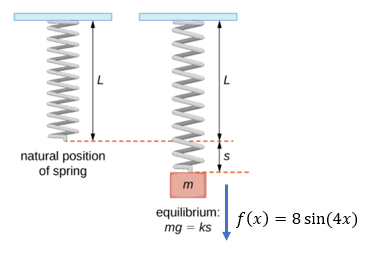
\includegraphics[width=6cm,height=4 cm]{diagram/spring2.PNG}
    \caption{Diagram shows the position of spring for the question that mention above}
    \label{fig1}
\end{figure}
\newpage
\section{Analytical Solution}
By using Equation \ref{eqn1}, we then can construct our ODEs from the given question. Our ODEs can be written as follow
\begin{align}
    my'' + by' + ky &= f(x)\\
    y'' + 8y' + 16y &= 8\;sin(4x) \label{eqn3}
\end{align}
Where in the given question, the value of mass, $m = 1$, damped force, $b = 8$ and spring constant, $k = 16$. From now, we can obtain the exact solution as
\begin{equation}\label{eqn4}
    y(x) = \frac{1}{4}e^{-4x} + xe^{-4x} - \frac{1}{4}cos(4x)
\end{equation}
Using Desmos graphic calculator, we can obtain the exact plot from Eyquation \ref{eqn4}. 
\begin{figure}[h]
    \centering
    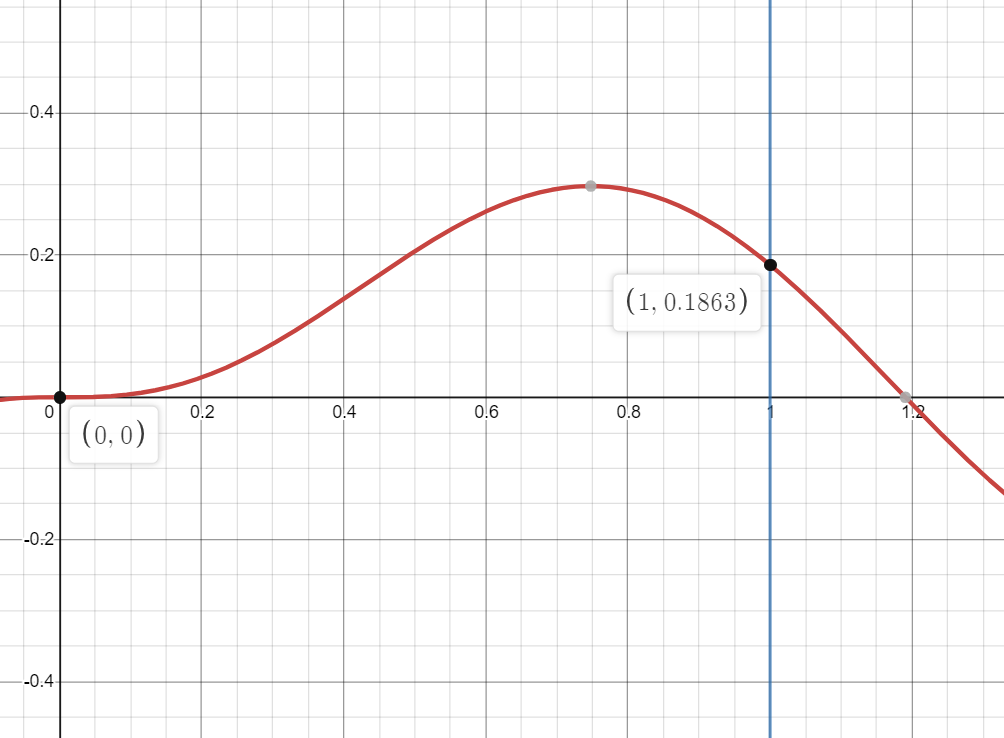
\includegraphics[width=6cm,height=4cm]{diagram/plot between 0 and 1.PNG}
    \caption{The exact plot that was obtain from Desmos calculator. In this figure, we only specify the boundary between $x=0$ and $x=1$, where it will be used in our numerical calculation and for Finite Difference method, we need to specify our boundary which are referred to the starting point and end point }
    \label{fig:my_label}
\end{figure}
\section{Numerical Solution}
In order to solve this problem numerically, I have applied Finite Difference method. The program to solve this problem was written in Python Language. The general form for ODEs which I applied in my coding can be written as follow 
\begin{equation}\label{eqnum}
    x''-p(x)x'-q(x)x = f(x)
\end{equation}
and we can compare Equation \ref{eqnum} with the Equation \ref{eqn3} to obtain their respective values/functions. Then, we can obtain their respective values as follow; $p(x) = -8$, $q(x) = -16$ and $f(x) = 8\;sin(4x)$. The Finite Difference method is a method where we transform our ODEs into tridiagonal matrix ($Ax = B)$, A and B is a matrix and x is referred to our solution. The reason why we transform our ODEs in tridiagonal matrix, so that it can be solve numerically. Below is the coding that I write to solve this ODEs. You can also run this code by clicking  \href{https://colab.research.google.com/drive/1UfvaS4Z1WwThruj0EPfhFcVaZ2bx0lt2?usp=sharing}{\textbf{here}}.
\begin{lstlisting}[language=Python, caption=Python code using Finite Difference Method to solve ODEs]
#Author: Ahmad Aiman B. Mohd Nazir (17060060)
from scipy.linalg import solve  #import the relevent libraries
import  numpy as np
import matplotlib.pyplot as plt
x = [0]      #set the initial value of x and define all parameters
f = []       #f(x)
n = 10       #number of iterations for n = 5,10,15,20,25,30 or mesh points
h = 1/n      #step size or increment
p = -8       #p(x)
q = -16      #q(x)
u = 0        #y(0)
u_1 = 0.1863   #y(1.0)

#define matrix zeros with size (n-1)x(n-1)
A = np.zeros((n-1,n-1))

#define matrix zeros with size (n-1)x(1)
B = np.zeros((n-1,1))

#append x values into array x by using loop
for i in range (0,n):
    x.append(x[i]+h)
    i+=1
#calculate the values of f(x) for each mesh points
for i in range (0,n):
  f.append(8*np.sin(4*x[i]))
  i+=1
#calculate the coefficient for tridiagonal matrix
a = 2+ q*h**2
b = -(1-1/2*p*h)
c = -(1+1/2*p*h)
#input the values obtain from a,b and c into matrix A
for i in range(0,n-1):
    for j in range(0,n-1):
        if i == j:
            A[i][j] = a
        elif i<j and j-i==1:
            A[i][j] = b
        elif i>j and i-j==1:
            A[i][j] = c
        else:
            A[i][j] = 0
    j+=1
i+=1
#input the values into matrix B
for i in range(0,n-1):
    for j in range(0,1):
        if i == j:
            B[i][j] = (1+(1/2)*p*h)*u - h**2*f[i+1]
        elif i > j and i<= n-3:
            B[i][j] = -(h**2)*f[i+1]
        elif i > j and i == n-2:
            B[i][j] = (1-(1/2)*p*h)*u_1 - (h**2)*f[i+1]
    j+=1
i+=1
X = solve(A,B)              #solve matrix AX = B

#define new array for x, ranging from 0 to 1 with increment = h
xnew = np.arange(0,1.01,h)  
y1 = np.insert(X,0,0)           #insert value y = 0 into y1[0]
ynew = np.append(y1,0.1863)     #append value y = 0.1863 in y1 array

#plot the graph ynew vs xnew
plt.plot(xnew,ynew,'-og',label='Approximate solution')

#define the exact solution
def exact(x):
    return 1/4*np.exp(-4*x) + x*np.exp(-4*x) - 1/4*np.cos(4*x)
#list of values of x with increment of 0.01
xexact = list(np.arange(0.0,1.01,0.01))

#calculate the yexact values for each xexact
yexact = []
for i in xexact:
  yexact.append(exact(i))
  
#plot the graph between yexact and xexact
plt.plot(xexact,yexact,'-k',label='exact solution')
plt.legend()
plt.xlabel('x')
plt.ylabel('y(x)')
plt.title('Plot y(x) versus x for ODE: '"$y''+8y'+16y = 8sin(4x)$")
plt.show()

\end{lstlisting}
\section{Result and Conclusion}
\begin{figure}[htb] \label{result}
    \centering % <-- added
\begin{subfigure}{0.25\textwidth}
  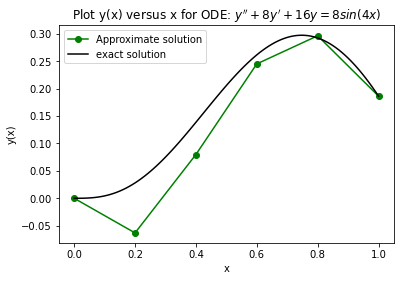
\includegraphics[width=\linewidth]{diagram/n=5.png}
  \caption{n = 5}
  \label{fig:1}
\end{subfigure}\hfil % <-- added
\begin{subfigure}{0.25\textwidth}
  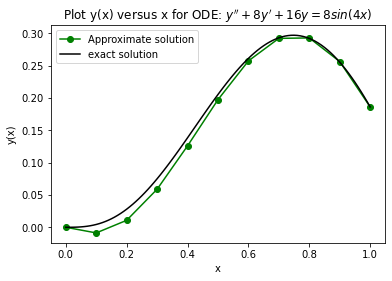
\includegraphics[width=\linewidth]{diagram/n = 10.png}
  \caption{n = 10}
  \label{fig:2}
\end{subfigure}\hfil % <-- added
\begin{subfigure}{0.25\textwidth}
  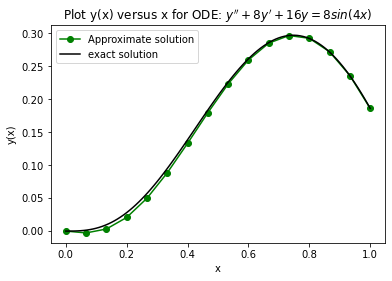
\includegraphics[width=\linewidth]{diagram/n = 15.png}
  \caption{n = 15}
  \label{fig:3}
\end{subfigure}

\medskip
\begin{subfigure}{0.25\textwidth}
  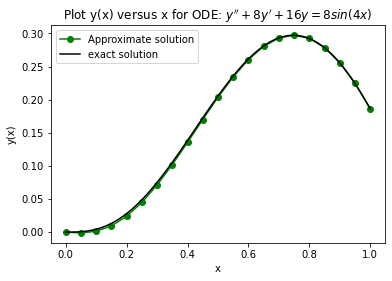
\includegraphics[width=\linewidth]{diagram/n = 20.png}
  \caption{n = 20}
  \label{fig:4}
\end{subfigure}\hfil % <-- added
\begin{subfigure}{0.25\textwidth}
  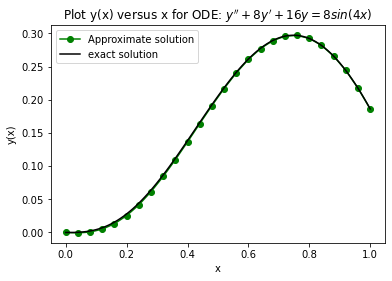
\includegraphics[width=\linewidth]{diagram/n = 25.png}
  \caption{n = 25}
  \label{fig:5}
\end{subfigure}\hfil % <-- added
\begin{subfigure}{0.25\textwidth}
  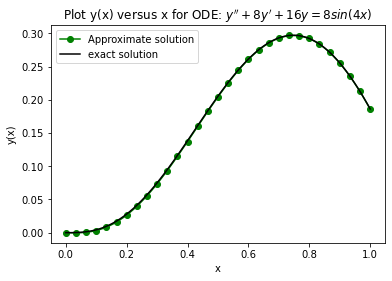
\includegraphics[width=\linewidth]{diagram/n = 30.png}
  \caption{n = 30}
  \label{fig:6}
\end{subfigure}
\caption{A few plots that represents the output of code }
\label{fig:images}
\end{figure}

Based on Figure 3, 6 difference plots were obtained for different numbers of iterations or mesh points, denoted as n. We can see as we increase the number of mesh points, n the approximate plot (green line) will be same as the exact plot (black line). Thus, we can conclude that Finite Difference method is one of the methods used in numerical calculation where we can solve the ordinary differential equations and it can give us a good approximation to the exact solution if the number of iterations or mesh points that we inputted into our coding is good enough or sufficient to approximate our solution. In Figure 4, we calculate the error for each mesh points between exact and approximate values for $n = 20$. Thus, we can conclude the error between approximate solution with exact solution is low, and the accuracy is increase if the number of iteration, n is large. 
\begin{figure}[h]
    \centering
    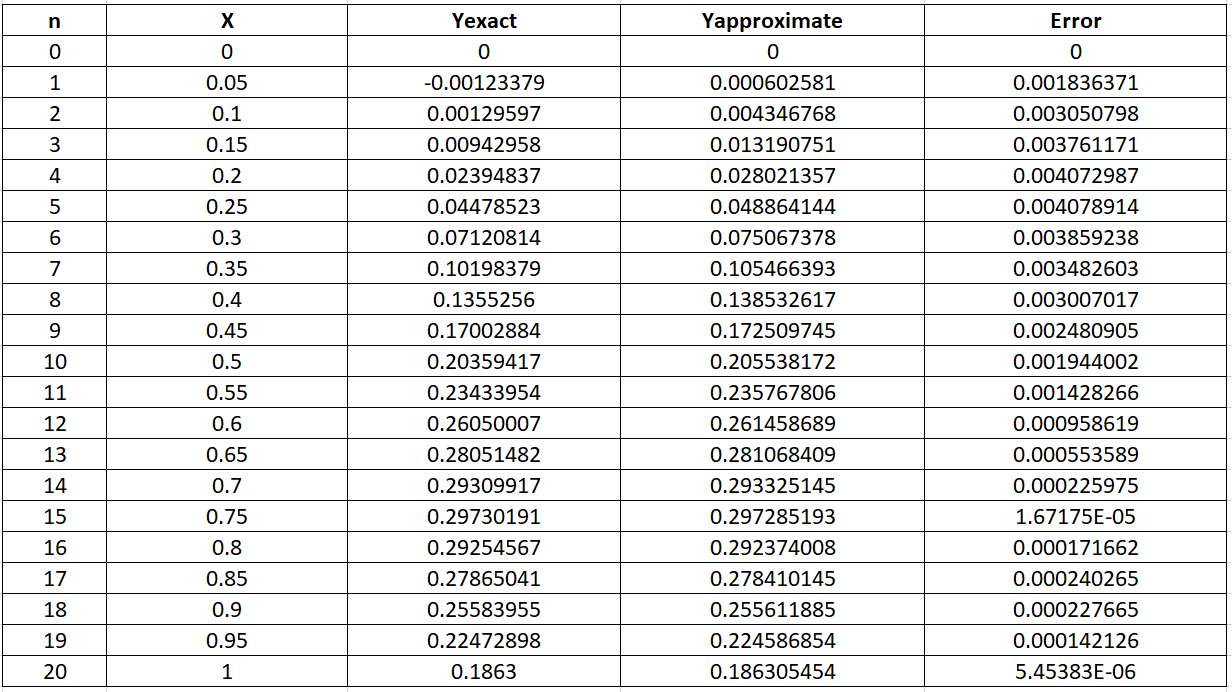
\includegraphics[width=12cm,height=8cm]{diagram/error.PNG}
    \caption{The error calculation for $n = 20$, error can be calculated by using $Y_{exact} - Y_{approximate}$ and we could see the range of our error in range of $10^{-3} - 10^{-6}$ which means our approximate value is quite accurate with the exact value}
\end{figure}

\bibliography{references}
\bibliographystyle{apacite}

\end{document}
